% multiple1902 <multiple1902@gmail.com>
% intro.tex
% Copyright 2011~2012, multiple1902 (Weisi Dai)
% https://code.google.com/p/xjtuthesis/
%
% It is strongly recommended that you read documentations located at
%   http://code.google.com/p/xjtuthesis/wiki/Landing?tm=6
% in advance of your compilation if you have not read them before.
%
% This work may be distributed and/or modified under the
% conditions of the LaTeX Project Public License, either version 1.3
% of this license or (at your option) any later version.
% The latest version of this license is in
%   http://www.latex-project.org/lppl.txt
% and version 1.3 or later is part of all distributions of LaTeX
% version 2005/12/01 or later.
%
% This work has the LPPL maintenance status `maintained'.
%
% The Current Maintainer of this work is Weisi Dai.
%

\chapter{基于二叉树搜索的文字检测方法}
\echapter{Text detection based on Binary Tree Search}

    \section{问题的提出}
    \esection{Questions Posed}

    \section{方法原理与步骤}
    \esection{Principle and Summary of The Method}



    \section{候选文字行的提取}
    \esection{Candidate text line's extraction}

        \subsection{统计边缘响应}
        \esubsection{Static Skeleton Response}

        首先提出统计边缘响应方法,用以增强文本与背景之间的响应强度差异。给定如图\ref{fig.c4_static_skeleton_response}(a) 所示的场景文字图像$g$,计算其统计边缘响应$s$ 的方式如算法\ref{alg:c4_static_skeleton_response} 所示:

        \begin{algorithm} \renewcommand{\algorithmicrequire}{\textbf{输入:}}	\renewcommand{\algorithmicensure}{\textbf{输出:}}
    	\caption{统计边缘响应}
    	\label{alg:c4_static_skeleton_response}
    	\begin{algorithmic}[1]
    		\REQUIRE 输入的场景文字图像$g$
    		\ENSURE 图$g$相对应的统计边缘响应$s$
            \STATE 在图$g$上利用基于边缘骨架切割的文字检测子得到粗略的定位结果:文字定位包围框集合$B$及其相应的置信度分数集合$C$
    		\REPEAT
            \STATE $rs:=\left\{ b \times c  |\,b \in B, c \in C\right\}$
            \STATE $s:=s\cup rs,B:=B / b,C:=C / c$
            \UNTIL{$B=\varnothing$}
    	\end{algorithmic}
        \end{algorithm}

        其中$rs$指代的是响应小块,它的底面积是1个定位包围框$b$,而高是$b$对应的置信度分数$c$。将所有的这些响应小块$rs$堆叠在一起,就构成了如图\ref{fig.c4_static_skeleton_response}(b) 所示的统计边缘响应$s$。

        \begin{figure}[htbp]
        \begin{minipage}[t]{0.37\linewidth}
        \centering
        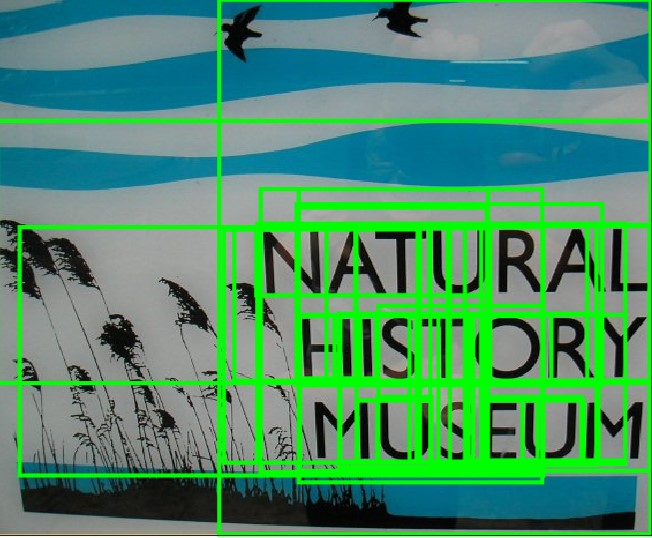
\includegraphics[width=\textwidth]{./figures/c4_img.jpg}
        \centerline{\small (a)粗略定位结果}
        \end{minipage}
        \begin{minipage}[t]{0.35\linewidth}
        \centering
        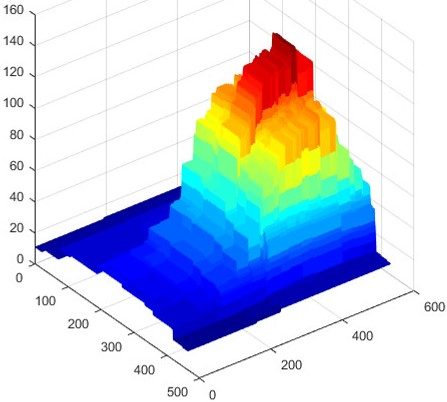
\includegraphics[width=\textwidth]{./figures/c4_static_skeleton_response.jpg}
        \centerline{\small (b)统计边缘响应}
        \end{minipage}
        \begin{minipage}[t]{0.25\linewidth}
        \centering
        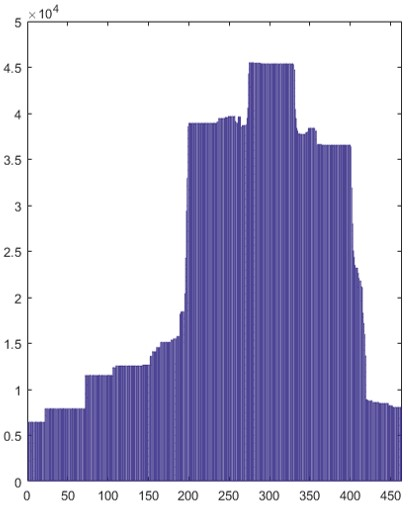
\includegraphics[width=\textwidth]{./figures/c4_horizontal_projection.jpg}
        \centerline{\small (c)水平方向的映射}
        \end{minipage}
        \caption{在统计边缘响应中,文本区域与背景可以被区分开;而且通过后续的对统计边缘响应的水平映射操作,文本行也可以进一步区分开彼此}
        \label{fig.c4_static_skeleton_response}
        \end{figure}

        为了后续提取候选文本行的操作,首先要利用公式\ref{eq:c4_horizontal_projection} 来计算统计边缘响应$s$的水平映射$hp$,如图\ref{fig.c4_static_skeleton_response}(c) 所示。

        \begin{equation}
        hp= \left\{ \sum_{j=1}^w s_{ij} \, | \, i=1,2,...,h;j=1,2,...,w \right\},
        \label{eq:c4_horizontal_projection}
        \end{equation}

        其中,$h,w$分别是统计边缘响应$s$的高度和宽度。

        \subsection{候选文字行的生成}
        \esubsection{Text line's construction}

        \begin{figure}[htbp]
        \begin{minipage}[t]{0.32\linewidth}
        \centering
        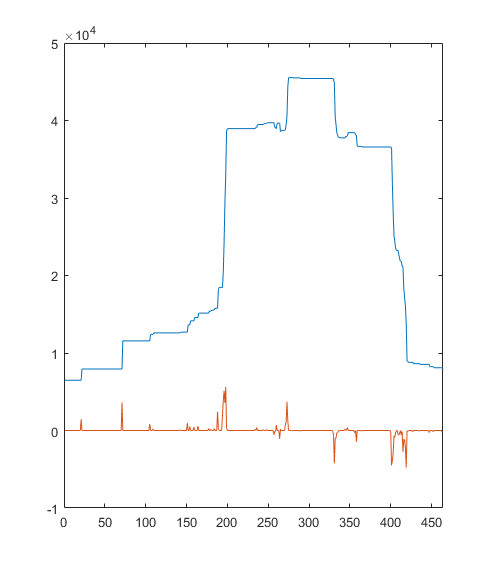
\includegraphics[width=\textwidth]{./figures/c4_gradient.jpg}
        \centerline{\small (a)在水平映射图上的梯度}
        \end{minipage}
        \begin{minipage}[t]{0.32\linewidth}
        \centering
        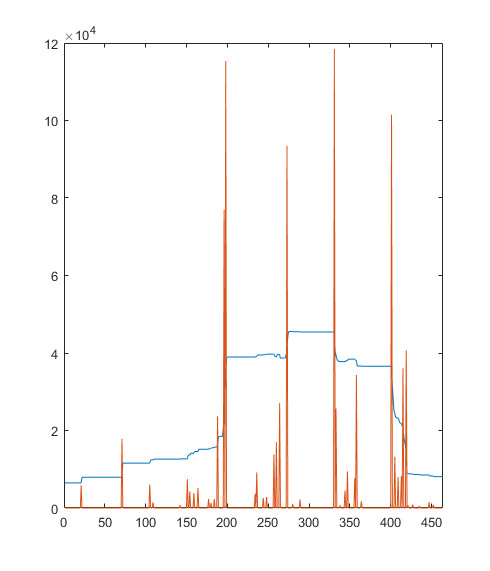
\includegraphics[width=\textwidth]{./figures/c4_unified.jpg}
        \centerline{\small (b)梯度的取正和统一坐标}
        \end{minipage}
        \begin{minipage}[t]{0.32\linewidth}
        \centering
        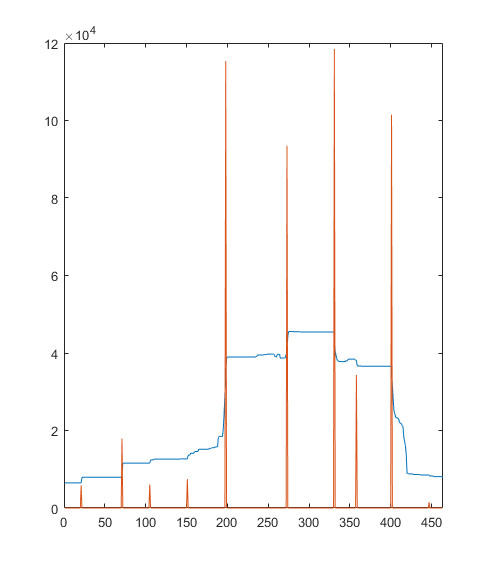
\includegraphics[width=\textwidth]{./figures/c4_nms.jpg}
        \centerline{\small (c)梯度的非极大值抑制}
        \end{minipage}
        \caption{通过梯度计算和非极大值抑制操作来粗略定位文本行}
        \label{fig.c4_candidate_line_construction}
        \end{figure}

    \section{二叉树型的文字行搜索空间的构建}
    \esection{Binary Tree-based search space's construction}

    \section{搜索最优的文字行定位}
    \esection{Searching the optimal text detection}

        \subsection{搜索路径}
        \esubsection{Searching the paths}

        \subsection{搜索策略}
        \esubsection{Searching strategies}

    \section{实验和结果分析}
    \esection{Experimental Results}

        \subsection{实验数据集与评价标准}
        \esubsection{Data-set and Evaluation Protocol}

        \subsection{实验结果与分析}
        \esubsection{Experimental Results and Analysis}

    \section{本章小结}
    \esection{Brief Summary}


